\documentclass{beamer}
\usetheme{Madrid}
\usepackage{cutwin}
\usepackage{tcolorbox}
\tcbuselibrary{fitting}
\usepackage{algorithmic}
\usepackage[linesnumbered,ruled,vlined]{algorithm2e}

\usepackage{lipsum}
\usepackage{subfig}
\tcbset{colframe=white,colback=white,
boxsep=0pt,top=1mm,bottom=1mm,left=1mm,right=1mm,
nobeforeafter,width=\linewidth}

\usepackage[style=authortitle,backend=bibtex]{biblatex}
\addbibresource{ref.bib}
\renewcommand{\footnotesize}{\scriptsize}

\author{Xiaofang Wang}
\title{Vision Domain Adaptation}
\institute{Ecole Centrale de Lyon \\ LIRIS}

% logo of my university
\titlegraphic{
\includegraphics[width=5cm]{figs/ecl.jpg}\hspace*{1cm}~%
   
\includegraphics[width=3cm]{figs/logo.jpg}
}





\begin{document}

\begin{frame}
\titlepage
\end{frame}
%============================
\begin{frame}
\frametitle{Outline} 
\tableofcontents 
\end{frame}
%============================
\section{Introduction to transfer learning} 
\subsection{Definition}
\begin{frame}{Transfer learning}
\begin{block}{Definition}
Ability of a system to recognize and apply knowledge and skills learned in
previous domains/tasks to novel domains/tasks \footfullcite{2010survey}
\end{block}
\begin{block}{Traditional
Machine Learning and Transfer Learning}
\begin{figure}
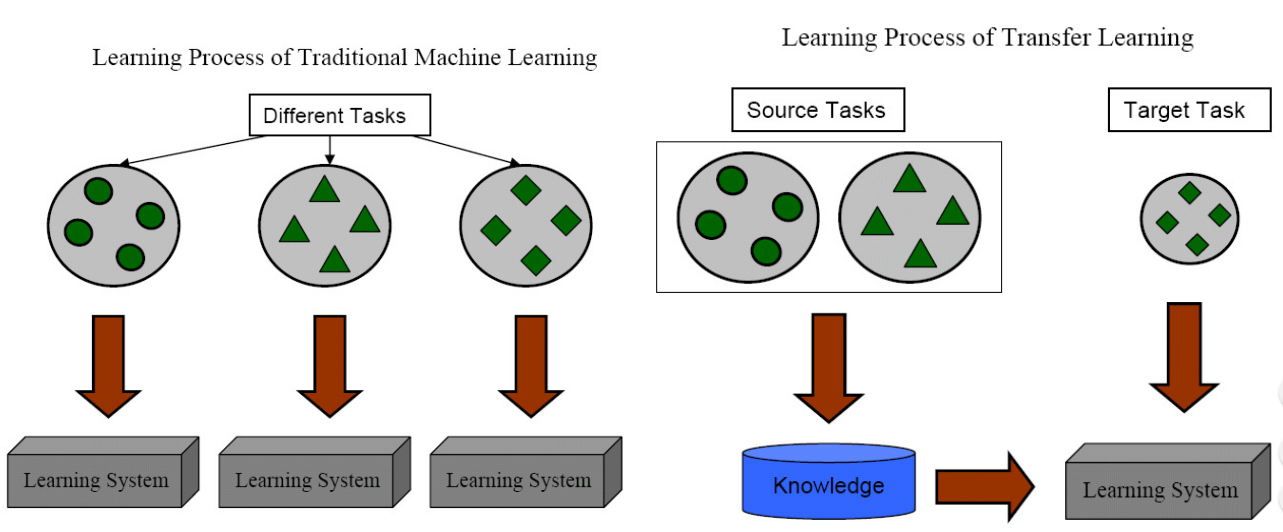
\includegraphics[width=0.7\textwidth]{figs/f3.png}
\end{figure}
\end{block}
\end{frame}
 \begin{frame}{Data mismatch in  image classification}
% $\Rightarrow$ Motivation examples: image classification dataset mismatch
    \begin{center}
  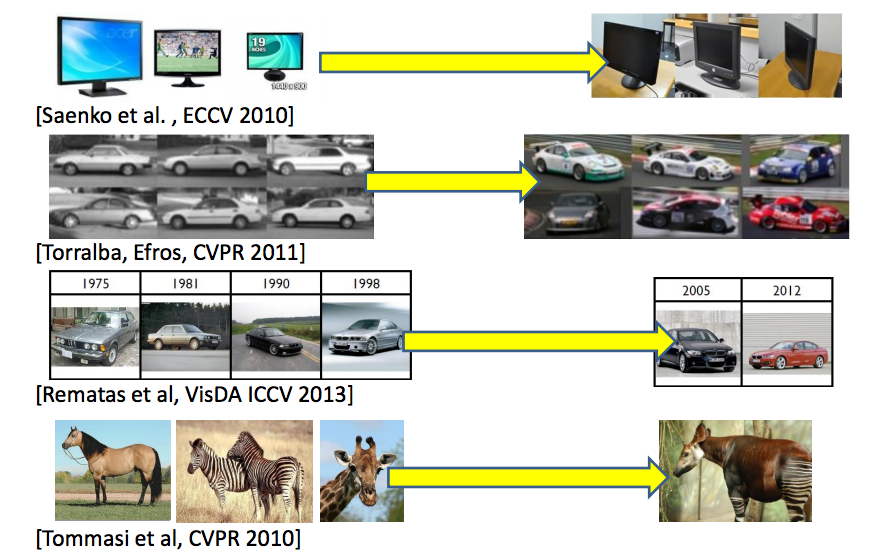
\includegraphics[width=0.8\textwidth]{figs/f5.png}
    \end{center}
$\Rightarrow$  Underlying causes: \\
different point of views, acquisition time and conditions,
\end{frame}
\begin{frame}{Motivation examples: Data mismatch in various vision tasks}
\begin{figure}
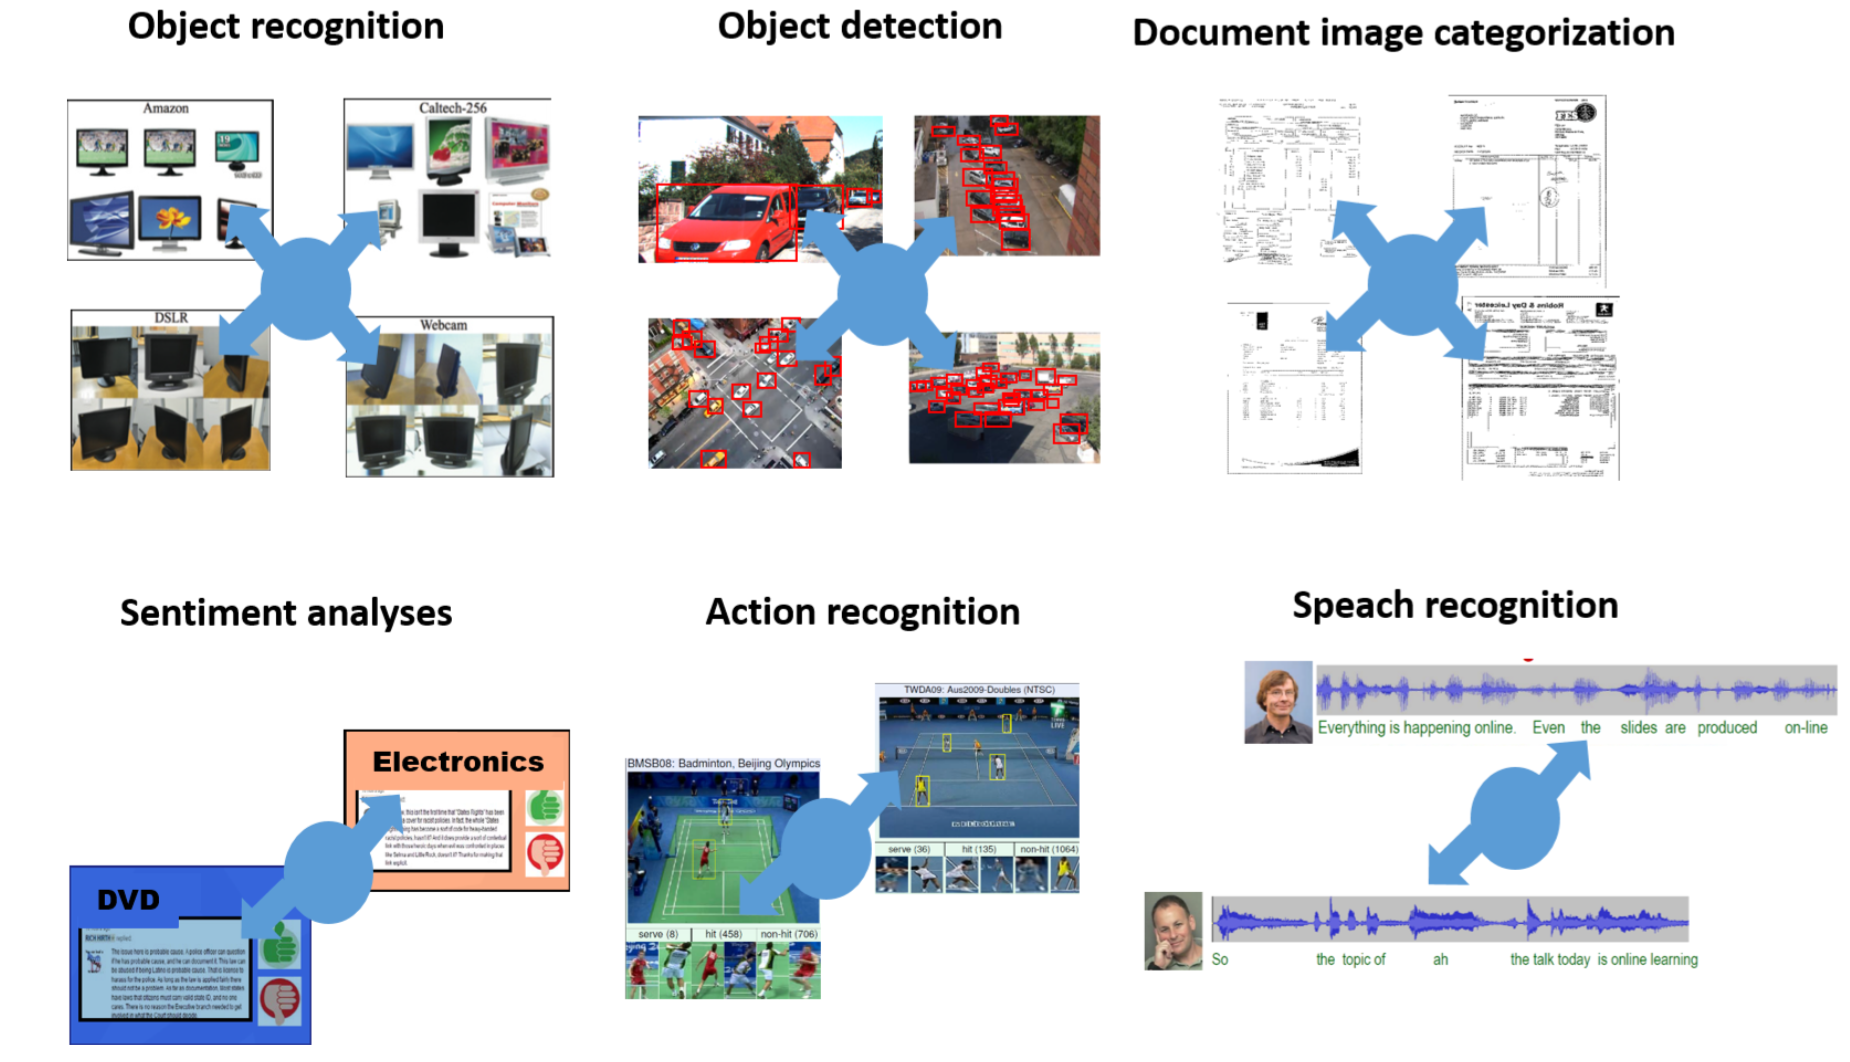
\includegraphics[width=0.9\textwidth]{figs/m2.png}
\end{figure}
\footnote{Image Courtesy to G. Csurka, DA for Visual Applications}
\end{frame}
\begin{frame}{ Data mismatch in various vision tasks}
\begin{block}{Underlying causes: }
\begin{itemize}
\item Audio recognition: different persons, environment, recording quality
\item Document image categorization: differences in appearance, layout
\item Activity recognition: different persons, environment, context
\item  Semantic analyses: different topics, vocabularies, ...
\end{itemize}
\end{block}
\end{frame}

%==================================
\subsection{Overview of transfer learning setting}
\begin{frame}{Overview of transfer learning setting}
\begin{figure}
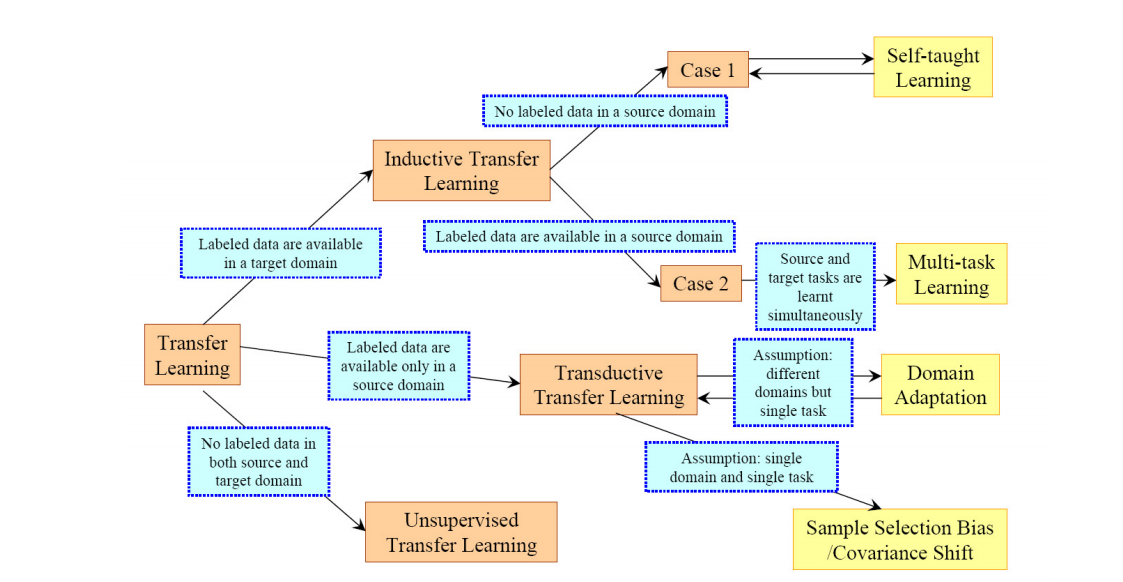
\includegraphics[width=\textwidth]{figs/f2.png}
\end{figure}
\footnote{Image Courtesy to \textcite{2010survey}}
\end{frame}

%=============================
\section{In this presentation}
\begin{frame}{In this presentation}
$\Rightarrow$  We will focus on:
\begin{itemize}
\item transfer learning setting: domain adaptation
\item  transfer task: image classification 
\item  transfer method: Feature-representation-transfer
\end{itemize}

$\Rightarrow$ Why?
\begin{itemize}
\item \textcolor{red}{Intensively concerned question}:  How can we learn, using labeled data from a source distribution, a low-error classifier for another related target distribution
\item \textcolor{red}{"Hot topic"}
\begin{itemize}
\item Tutorials at ICML 2010, CVPR 2012, Interspeech 2012, ECCV 2014
\item Workshops at NIPS 2005 Workshop, NIPS 2006, AAAI 2008, NIPS 2009, ICDM 2009, ACL 2010 Workshop.


\end{itemize}

\end{itemize}
\end{frame}
%==========================
\section{Domain adaptation}
\subsection{Domain adaptation:Definition and settings}
\begin{frame}{Domain adaptation}
\begin{columns}[totalwidth=\textwidth]
\begin{column}{\textwidth}

\tcboxfit[height=4cm]{
\begin{block}{Notations}
\begin{table}
\centering
\begin{tabular}{|c|l|}
\hline
$\chi \in \mathcal X$ & Input variable to a learning system (i.e. observation)\\
\hline
$y \in \mathcal Y$ & Output variable to a learning system (i.e. label) \\ \hline
$\mathcal{X}, \mathcal{Y}$ & Feature and Label Space \\ \hline
$\mathcal{D}= \{ \mathcal{X}, P(\mathcal{X}) \}$ & \textbf{Domain}: pair of feature space and  marginal
distribution. \\ \hline
$\mathcal{T}=\{\mathcal{Y}, P(\mathcal{Y}|\mathcal{X})\}$ & \textbf{Task}: pair of label space and conditional probability.\\ \hline
\end{tabular}
\end{table}
\end{block}


}
\end{column}
\end{columns}

\begin{block}{Unsupervised domain adaptation}
Source with large amount of labeled data.
 Target with no labels.
\end{block}
\begin{block}{Semi-supervised domain adaptation}
Source with large amount of labeled data.
 Target with a limited amount of labels.
\end{block}
\end{frame}

\subsection{Problem definition}
\begin{frame}{Problem definition}

\begin{columns}[totalwidth=\textwidth]
\begin{column}{\textwidth}

\tcboxfit[height=0.9\textheight]{
\begin{block}{Settings}
Given with:
\begin{itemize}
\item $ \mathcal S = \{(x_i , y_i )\}_{i=1}^{n_s}$  Source sample drawn i.i.d. from $P_S(X)$
\item $\mathcal T = \{x_j \}_{j=1}^{n_t}$ Target Sample drawn i.i.d. from $P_T(X)$
\end{itemize}

\begin{table}
\centering
\begin{tabular}{|c|l|}
\hline
$\mathcal{D}_S \neq \mathcal{D}_T $ & Source domain and target domain are different\\
\hline

$P_S(\mathcal X) \neq P_S(\mathcal X)$ &  marginal probability are different \\ \hline

$ P_S(\mathcal{Y}|\mathcal{X}) \neq P_T(\mathcal{Y}|\mathcal{X})$& conditional probability are different\\ \hline
$\mathcal Y_S = \mathcal Y_T$ & their tasks are the same \\ \hline
\end{tabular}
\end{table}
\end{block}

}

\end{column}
\end{columns}

\end{frame}
%============================

\subsection{Problem definition: what,how,and When?}
\begin{frame}{Problem definition: what,how,and When?}

\begin{itemize}
\item \textcolor{red}{What}: Define the knowledge that should be extracted from the
source and used on the target.
\begin{figure}
 \centering
\subfloat[Instances\label{fig:1}]{
    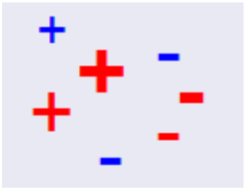
\includegraphics[height=2cm]{figs/f6_1.png}}
\subfloat[Model\label{fig:2}]{
    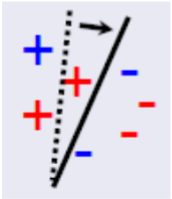
\includegraphics[height=2cm]{figs/f6_2.png}}
    \subfloat[Feature \label{fig:3}]{
   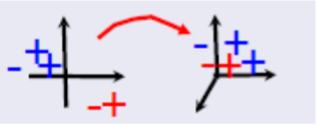
\includegraphics[height=2cm]{figs/f6_3.png}}
    
\end{figure}

\end{itemize}
\end{frame}

\begin{frame}{Proble definition: What, how and when?}

\begin{itemize}

\item \textcolor{red}{How}: Define the algorithm that extract this knowledge and
leverages over it.
\begin{block}{Instance-based method}
Correct a sample bias by reweighting source labeled data
\end{block}
\begin{block}{Adjust methods}
Modify the model by incorporating+pseudo-labeled information
\end{block}
\begin{block}{Feature based methods}
Find a common space where source and target are close
(projection, new features, etc)
\end{block}

\end{itemize}
\end{frame}

\begin{frame}{feature-based representation}
\begin{columns}[totalwidth=\textwidth]
\begin{column}{\textwidth}
% $\Rightarrow$ Definition\\
\tcboxfit[height=\textheight]{
\begin{center}
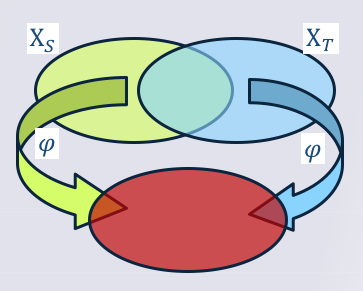
\includegraphics[height=0.3\textheight]{figs/f7.png}
\end{center}
$\Rightarrow$ \textcolor{red}{When source and target domains only have some overlapping features. (lots of features only have support in either the source or the target domain)} \\
$\Rightarrow$ How to learn $\phi$?
\begin{itemize}
\item Solution 1: Encode application-specific knowledge to learn the transformation.
\begin{itemize}
\item Source domain  specific features;
 \item Target domain  specific features;
 \item  Domain independent features (pivot features)
\end{itemize}
\end{itemize}
}
\end{column}

\end{columns}
\end{frame}


\begin{frame}{Feature-based transfer}
\begin{columns}[totalwidth=\textwidth]
\begin{column}{\textwidth}
% $\Rightarrow$ Definition\\
\tcboxfit[height=\textheight]{
\begin{center}
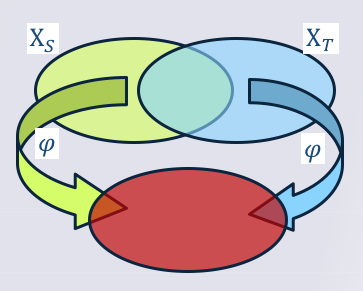
\includegraphics[height=0.3\textheight]{figs/f7.png}
\end{center}
$\Rightarrow$ \textcolor{red}{ How to identify pivot features?}
\begin{itemize}
\item Term frequency on both domains
\item Mutual information between features and labels (source domain) \item Mutual information on between features and domains
\end{itemize}
$\Rightarrow$ \textcolor{red}{ How to utilize pivots to align features across domains?}
\begin{itemize}
\item Structural Correspondence Learning (SCL) [Biltzer etal.
EMNLP-06]
 \item Spectral Feature Alignment (SFA) [Pan etal. WWW-10]
\end{itemize}}
\end{column}
\end{columns}
\end{frame}


%==================
\begin{frame}{Feature-based transfer}
\begin{columns}[totalwidth=\textwidth]
\begin{column}{\textwidth}
\tcboxfit[height=\textheight]{
\begin{center}
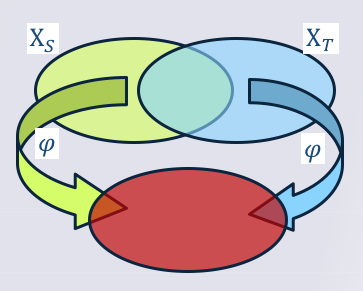
\includegraphics[height=0.4\textheight]{figs/f7.png}
\end{center}
$\Rightarrow$ \textcolor{red}{ How to learn $\phi$ ?}
\begin{itemize}
\item Solution 2: General approaches to learning the transformation. 
\begin{itemize}
\item Learning features by minimizing distance between distributions
\item Learning features inspired by multi-task learning
 \item Learning features inspired by self-taught learning
\end{itemize}
\end{itemize}}
\end{column}
\end{columns}
\end{frame}

%==================
\begin{frame}{Feature-based representation transfer}

\begin{minipage}[0.1\textheight]{\textwidth}
\begin{columns}[totalwidth=\textwidth]
\begin{column}{0.8\textwidth}
$\Rightarrow$ \textcolor{red}{ "Learning features by minimizing distance between distributions" }
\end{column}
\begin{column}{0.2\textwidth}
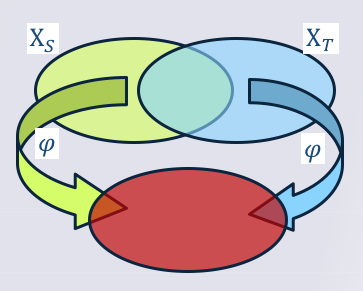
\includegraphics[width=2.5cm]{figs/f7.png}
\end{column}
\end{columns}
\end{minipage}
\tcboxfit[height=0.57\textheight]{
\begin{itemize}
 \item \textbf{Transfer Component Analysis(TCA)} [\textcite{pan2011domain}]
\item \textbf{Joint Domain Adaptation(JDA)} [\textcite{long2013transfer}]
 \item \textbf{Geodesic Flow Sampling(GFS)}[\textcite{gong2012geodesic}]
 \item \textbf{Geodesic Flow Kernel(GFK)} [\textcite{gong2012geodesic}]
 \item \textbf{Subspace Alignment(SA)} [\textcite{fernando2013unsupervised}]
 \item \textbf{Our proposal: Close yet Distinctive Domain Adaptation (CDDA)} [\textcite{luo2017close}]
 \item \textbf{Our proposal: Robust Data Geometric Structure Aligned Close yet Discriminative Domain Adaptation (RSA-CDDA)} [\textcite{luo2017robust}]
 \end{itemize}
 }
\end{frame}

\begin{frame}{Feature-based representation transfer}

\begin{minipage}[0.1\textheight]{\textwidth}
\begin{columns}[totalwidth=\textwidth]
\begin{column}{0.8\textwidth}
$\Rightarrow$ \textcolor{red}{ "Learning features by minimizing distance between distributions" }

$\Rightarrow$ \textcolor{red}{ Deep learning }
\end{column}
\begin{column}{0.2\textwidth}
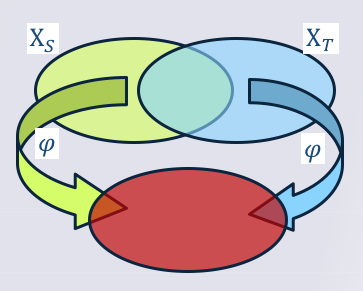
\includegraphics[width=2.5cm]{figs/f7.png}
\end{column}
\end{columns}
\end{minipage}
\tcboxfit[height=0.57\textheight]{
\begin{itemize}
\item DDC - Deep Domain Confusion, \footcite{tzeng2014deep}.
\item  DAN - Deep Adaptation Networks, \footcite{long2015learning}
\item  DAB Domain Adaptation by Backpropagation, \footcite{ganin2015unsupervised}

 \end{itemize}
 }
\end{frame}




\section{Our proposal I: CDDA}
\begin{frame}{Close yet Distinctive Domain Adaptation(CDDA)}
\small
\begin{block}{Motivation}
Find a common feature space where dependencies between domains are \textcolor{red}{minimized}, meanwhile intrinsic subdomain's \textcolor{red}{discriminative structure} is preserved. 
\end{block}
\begin{figure}
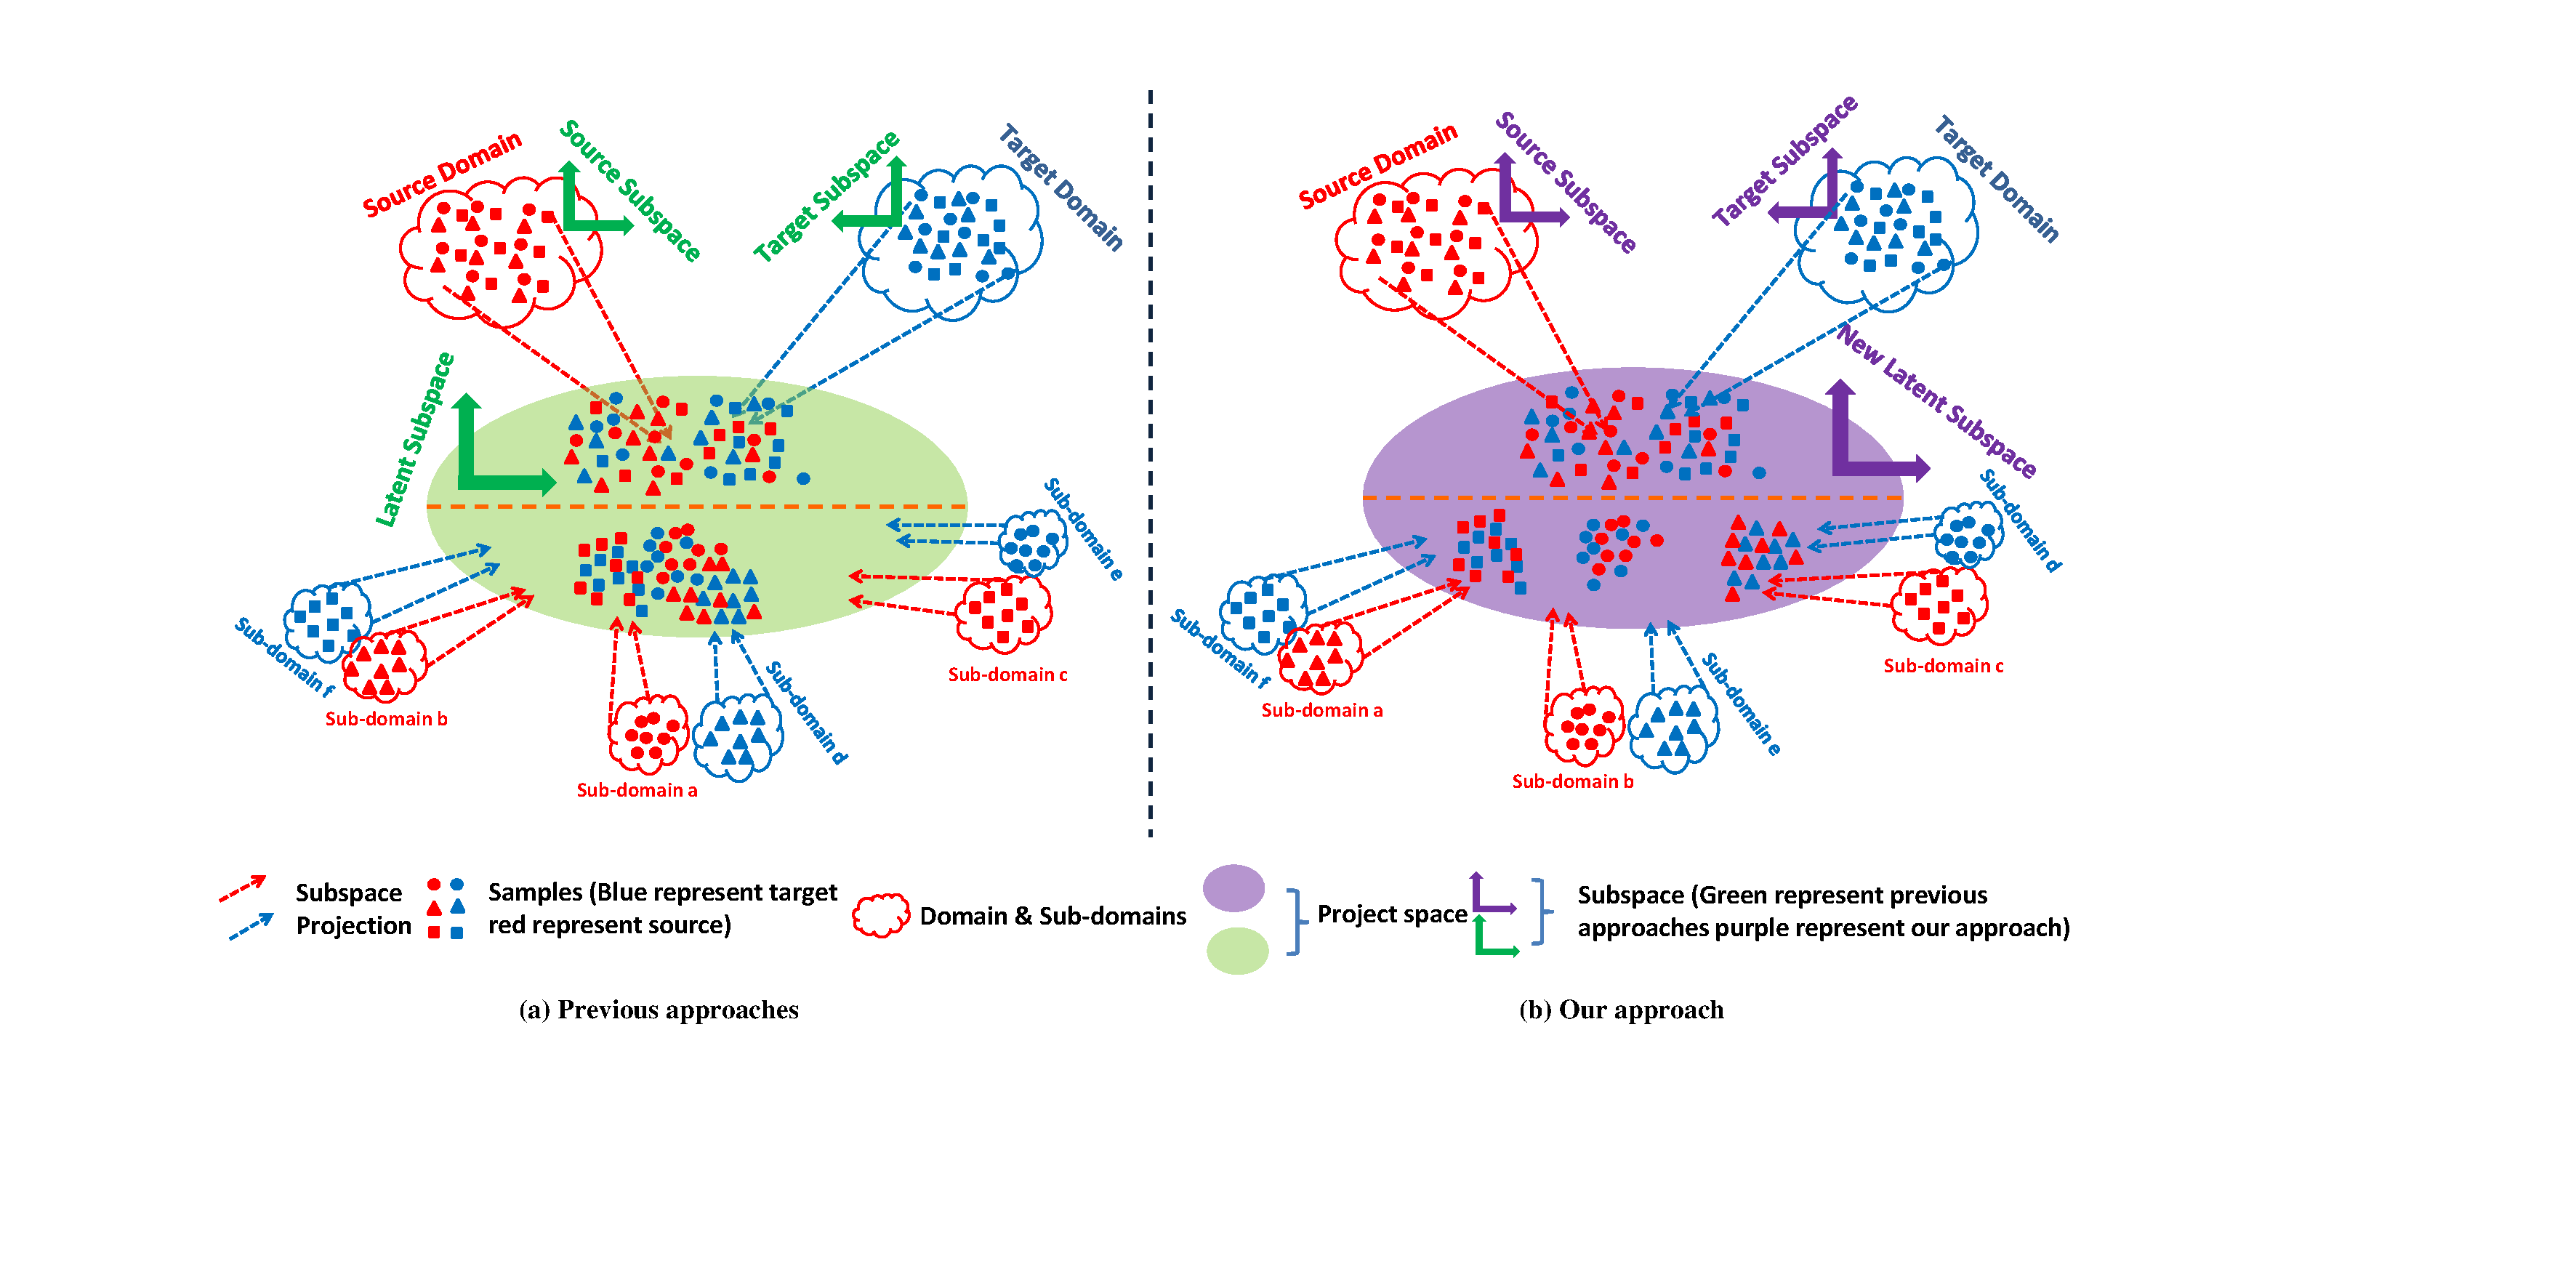
\includegraphics[width=0.9\textwidth]{figs/iccv.pdf}
\end{figure}
\end{frame}

%=======================
\begin{frame}{Optimization Function}
\begin{block}{CDDA model fomulaltion}
\begin{equation}\label{eq:ours_physical}
		\resizebox{0.96\hsize}{!}{%
	$\begin{array}{*{20}{l}}
		{\min (Dis{t^{marginal}} + Dis{t^{conditional}} + Dis{t^{label}} + {{\bf{Y}}^T}L{\bf{Y}})}\\ + 
		\max (Dist^{repulsive})
	\end{array}$}
\end{equation}

\begin{itemize}
\item $\min(Dis{t^{marginal}}+Dis{t^{conditional}})$: Marginal and conditional distribution are introduced in JDA \footcite{long2013transfer}
\item $\max (Dist^{repulsive})$: Our proposed repulsive term.  
\item $ Dis{t^{label}} + {{\bf{Y}}^T}L{\bf{Y}}$: Label propagation.
\end{itemize}
\end{block}
\textbf{Remark}:  \small{The MMD distance between distributions of two samples can be well-estimated by the distance between the means of the two samples mapped into a RKHS--- TCA} \footcite{pan2011domain}
\end{frame}
%=============================
\begin{frame}
{Maximum Mean Discrepancy (MMD)}
\begin{figure}
\centering
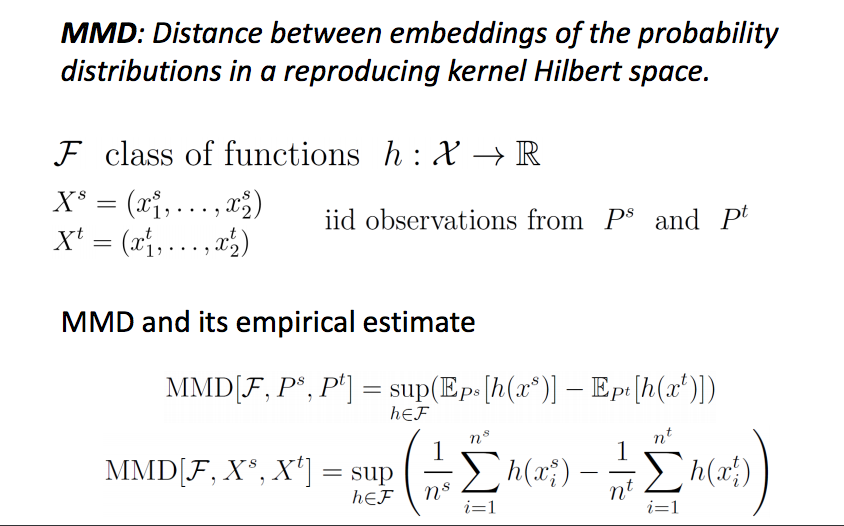
\includegraphics[width=\textwidth]{figs/MMD1.png}
\end{figure}
\footcite{borgwardt2006integrating}
\end{frame}
\begin{frame}
{Maximum Mean Discrepancy (MMD)}
\begin{figure}
\centering
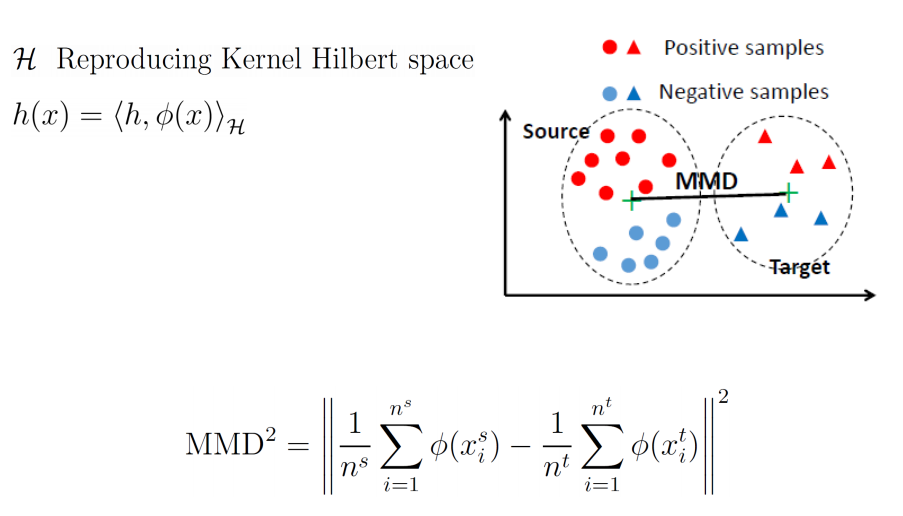
\includegraphics[width=\textwidth]{figs/MMD.png}
\end{figure}
\footcite{borgwardt2006integrating}
\end{frame}
%=================

%===================================
\begin{frame}{ Distance measurement}
Original data $\boldsymbol{X}$ is projected into the  optimal $k$-dimensional subspace using $\boldsymbol{Z} = \boldsymbol{A}^T\boldsymbol{X}$. 
here we define $\phi=\boldsymbol{Z} $, we write the MMD-RKHS distance represented by matrix: 
\begin{columns}[totalwidth=\textwidth]
\begin{column}{\textwidth}
\tcboxfit[height=0.8\textheight]
{
\begin{block}
{Marginal distribution distance}

\begin{equation}\label{eq:marginal}
	\begin{array}{l}		
		Dis{t^{marginal}}({{\cal D}_{\cal S}},{{\cal D}_{\cal T}}) ={\left\| {\frac{1}{{{n_s}}}\sum\limits_{i = 1}^{{n_s}} {{{\bf{A}}^T}{x_i} - } \frac{1}{{{n_t}}}\sum\limits_{j = {n_s} + 1}^{{n_s} + {n_t}} {{{\bf{A}}^T}{x_j}} } \right\|^2}
	\end{array}
\end{equation}
\end{block}
\begin{block}
{Conditional distribution}
\begin{equation}\label{eq:conditional}
		\begin{array}{c}
		\begin{array}{l}
		Dis{t^{conditional}}\sum\limits_{c = 1}^C {({{\cal D}_{\cal S}}^c,{{\cal D}_{\cal T}}^c)}  = 
		{\left\| {\frac{1}{{n_s^{(c)}}}\sum\limits_{{x_i} \in {{\cal D}_{\cal S}}^{(c)}} {{{\bf{A}}^T}{x_i}}  - \frac{1}{{n_t^{(c)}}}\sum\limits_{{x_j} \in {{\cal D}_{\cal T}}^{(c)}} {{{\bf{A}}^T}{x_j}} } \right\|^2}
		
		\end{array}
		\end{array}
\end{equation}
where $C$ is the number of classes, $\mathcal{D_S}^{(c)}$ represents the ${c^{th}}$ sub-domain in the source domain, $n_s^{(c)}$ is the number of samples in the ${c^{th}}$ {source} sub-domain. 
\end{block}
}
\end{column}
\end{columns}
\end{frame}


\begin{frame}{ Distance measurement}
\begin{columns}[totalwidth=\textwidth]
\begin{column}{\textwidth}
\tcboxfit[height=0.8\textheight]
{
\begin{block}{Repulsive Force Domain Adaptation}
\begin{equation}\label{eq:repulsive}
{Dist}^{repulsive} = {Dist}_{{\cal S} \to {\cal T}}^{repulsive}+{Dist}_{{\cal T} \to {\cal S}}^{repulsive}
\end{equation}
\end{block}

\begin{block}
{Repulsive distance S to T}
\begin{equation}\label{eq:StoT}
% 		\resizebox{1\hsize}{!}{%
			%$
 {Dist}_{{\cal S} \to {\cal T}}^{repulsive} = \sum\limits_{c = 1}^C \begin{array}{l}
			{\left\| {\frac{1}{{n_s^{(c)}}}\sum\limits_{{x_i} \in {D_{\cal S}}^{(c)}} {{{\bf{A}}^T}{x_i}}  - \frac{1}{{\sum\limits_{r \in \{ \{ 1...C\}  - \{ c\} \} } {n_t^{(r)}} }}\sum\limits_{{x_j} \in D_{\cal T}^{(r)}} {{{\bf{A}}^T}{x_j}} } \right\|^2}
			\end{array} %$}
	\end{equation}
\end{block}
\begin{block}
{Repulsive distance T to S}
\begin{equation}\label{eq:TtoS}
% 		\resizebox{1\hsize}{!}{%
Dist_{T \to S}^{repulsive} = \sum\limits_{c = 1}^C \begin{array}{l}
			{\left\| {\frac{1}{{n_s^{(c)}}}\sum\limits_{{x_i} \in {D_T}^{(c)}} {{{\bf{A}}^T}{x_i}}  - \frac{1}{{\sum\limits_{r \in \{ \{ 1...C\}  - \{ c\} \} } {n_t^{(r)}} }}\sum\limits_{{x_j} \in D_S^{(r)}} {{{\bf{A}}^T}{x_j}} } \right\|^2}
	\end{array}  
	\end{equation}
\end{block}
}
\end{column}
\end{columns}
\end{frame}


%==============
\begin{frame}
{How to minimize the MMD-RKHS distance}
\begin{block}
{Minimization MMD-RKHS}

\end{block}
\begin{figure}
\centering
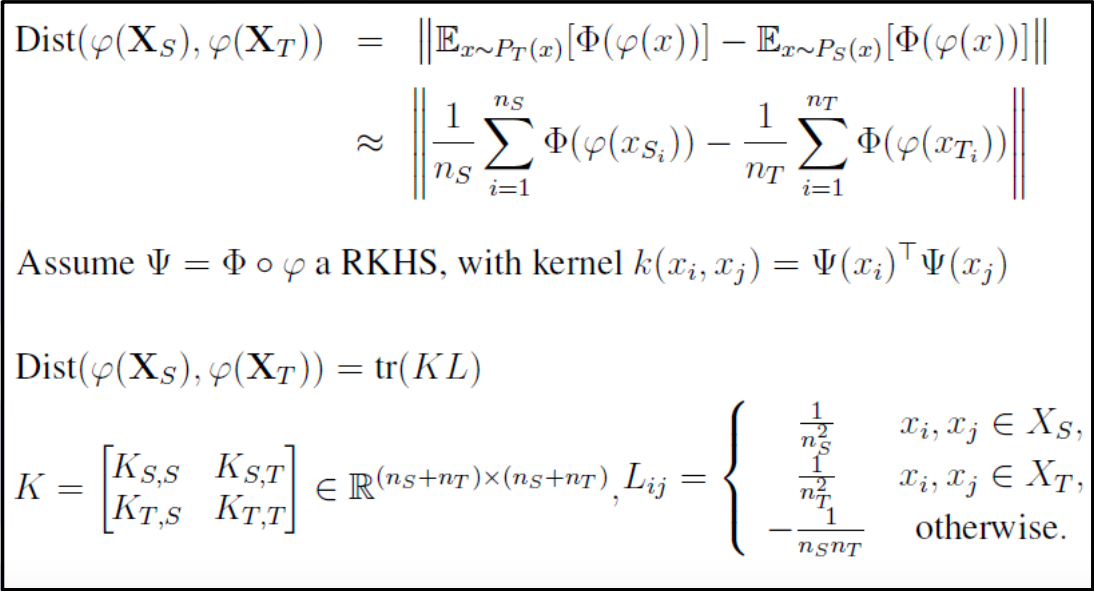
\includegraphics[width=0.8\textwidth]{figs/m1.png}
\end{figure}
\textcite{pan2008transfer}
\end{frame}
\begin{frame}
{How to minimize the MMD-RKHS distance}
\begin{figure}
\centering
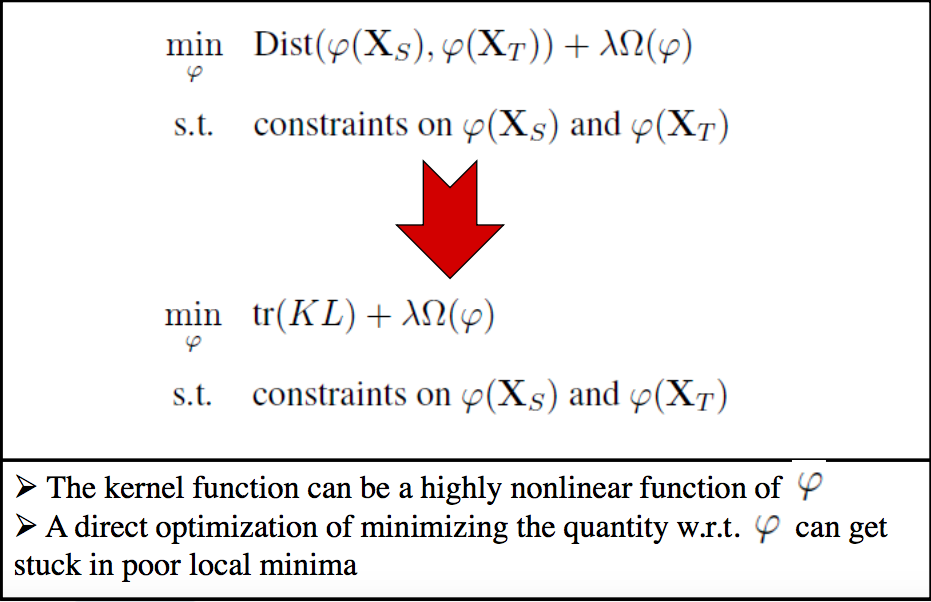
\includegraphics[width=0.8\textwidth]{figs/m11.png}
\end{figure}
\textcite{pan2008transfer}
\end{frame}
\begin{frame}
{How to minimize the MMD-RKHS distance}
\begin{figure}
\centering
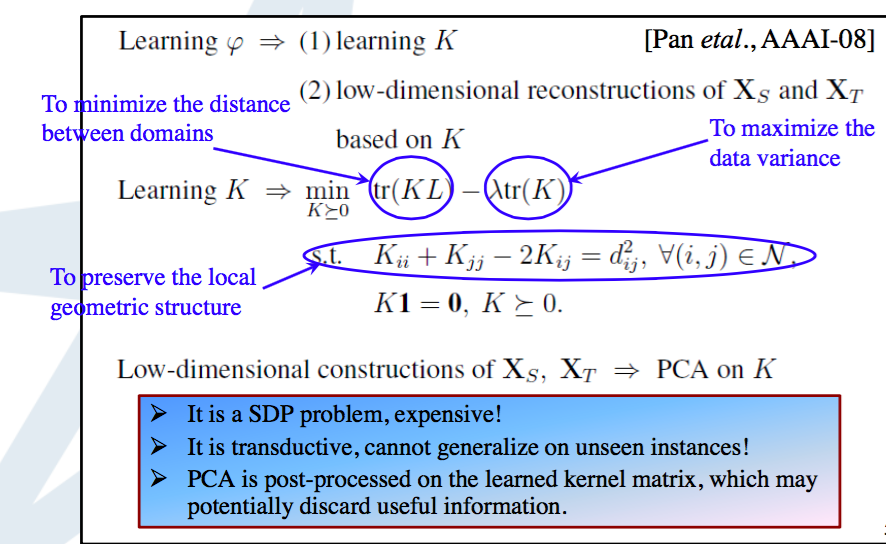
\includegraphics[width=0.8\textwidth]{figs/tca.png}
\end{figure}
\textcite{pan2011domain}
\end{frame}

\begin{frame}
{How to minimize the MMD-RKHS distance}
\begin{figure}
\centering
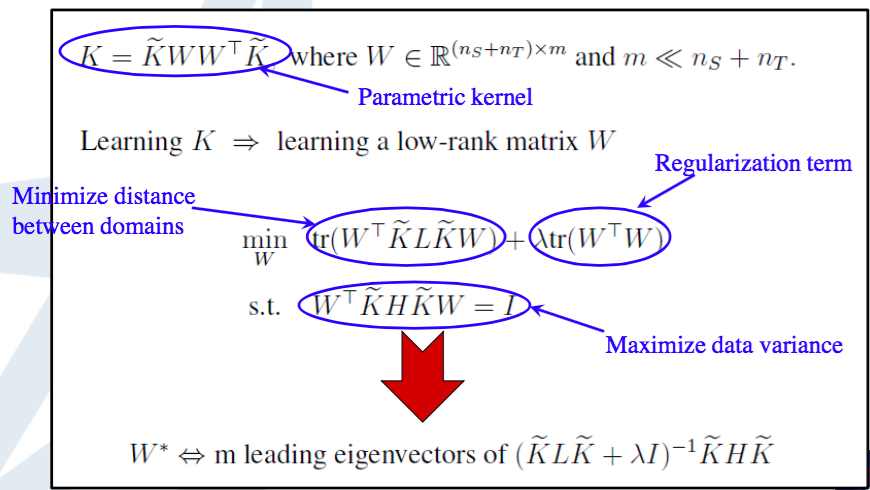
\includegraphics[width=0.8\textwidth]{figs/tca1.png}
\end{figure}
\textcite{pan2011domain}
\end{frame}

\begin{frame}{ Closer: Marginal and Conditional Distribution
Domain Adaptation}
\begin{columns}[totalwidth=\textwidth]
\begin{column}{\textwidth}
\tcboxfit[height=\textheight]
{
\begin{block}
{Marginal distribution minimization problem}

\begin{equation}\label{eq:marginal}
	\begin{array}{l}		
		Dis{t^{marginal}}({{\cal D}_{\cal S}},{{\cal D}_{\cal T}}) =\\ {\left\| {\frac{1}{{{n_s}}}\sum\limits_{i = 1}^{{n_s}} {{{\bf{A}}^T}{x_i} - } \frac{1}{{{n_t}}}\sum\limits_{j = {n_s} + 1}^{{n_s} + {n_t}} {{{\bf{A}}^T}{x_j}} } \right\|^2}
		= tr({{\bf{A}}^T}\bf{X}{\bf{M_0}}\bf{{X^T}A})		
		\end{array}
\end{equation}
where ${{\bf{M}}_0}$ represents the marginal distribution between ${{\cal D}_{\cal S}}$ and ${{\cal D}_{\cal T}}$ and its calculation is obtained by:
	
	\begin{equation}\label{eq:M0}
	\begin{array}{l}
	{({{\bf{M}}_0})_{ij}} = \left\{ \begin{array}{l}
	\frac{1}{{{n_s}{n_s}}},\;\;\;{x_i},{x_j} \in {D_{\cal S}}\\
	\frac{1}{{{n_t}{n_t}}},\;\;\;{x_i},{x_j} \in {D_{\cal T}}\\
	\frac{-1}{n_s n_t}\;\;\;otherwise
	\end{array} \right.
	\end{array}
	\end{equation}
   
\end{block}
}
\end{column}
\end{columns}
\end{frame}
%=================

\begin{frame}{Closer: Marginal and Conditional Distribution
Domain Adaptation}
\begin{columns}[totalwidth=\textwidth]
\begin{column}{\textwidth}
\tcboxfit[height=\textheight]{
\begin{block}
{Conditional distribution minimization problem }
\begin{equation}\label{eq:conditional}
		\begin{array}{c}
		\begin{array}{l}
		Dis{t^{conditional}}\sum\limits_{c = 1}^C {({{\cal D}_{\cal S}}^c,{{\cal D}_{\cal T}}^c)}  = \\
		{\left\| {\frac{1}{{n_s^{(c)}}}\sum\limits_{{x_i} \in {{\cal D}_{\cal S}}^{(c)}} {{{\bf{A}}^T}{x_i}}  - \frac{1}{{n_t^{(c)}}}\sum\limits_{{x_j} \in {{\cal D}_{\cal T}}^{(c)}} {{{\bf{A}}^T}{x_j}} } \right\|^2}
		= tr({{\bf{A}}^T}{\bf{X}}{{\bf{M}}_c}{{\bf{X}}^{\bf{T}}}{\bf{A}})
		\end{array}
		\end{array}
\end{equation}
where $C$ is the number of classes, $\mathcal{D_S}^{(c)}$ represents the ${c^{th}}$ sub-domain in the source domain, $n_s^{(c)}$ is the number of samples in the ${c^{th}}$ {source} sub-domain. 

\begin{equation}
\begin{array}{*{20}{c}}
{{{({{\bf{M}}_c})}_{ij}} = \left\{ {\begin{array}{*{20}{l}}
		{\frac{1}{{n_s^{(c)}n_s^{(c)}}},\;\;\;{x_i},{x_j} \in {D_{\cal S}}^{(c)}}\\
		{\frac{1}{{n_t^{(c)}n_t^{(c)}}},\;\;\;{x_i},{x_j} \in {D_{\cal T}}^{(c)}}\\
		{\frac{{ - 1}}{{n_s^{(c)}n_t^{(c)}}},\;\;\;\left\{ {\begin{array}{*{20}{l}}
				{{x_i} \in {D_{\cal S}}^{(c)},{x_j} \in {D_{\cal T}}^{(c)}}\\
				{{x_i} \in {D_{\cal T}}^{(c)},{x_j} \in {D_{\cal S}}^{(c)}}
				\end{array}} \right.}\\
		{0,\;\;\;\;\;\;\;\;\;\;\;\;otherwise}
		\end{array}} \right.}
\end{array}
\end{equation}
\end{block}
}
\end{column}
\end{columns}
\end{frame}


\begin{frame}{More discriminative:Repulsive Force Domain Adaptation}
\begin{columns}[totalwidth=\textwidth]
\begin{column}{\textwidth}
\tcboxfit[height=\textheight]{
\begin{block}{Repulsive Force Domain Adaptation: from $S \Rightarrow T$ }
\begin{equation}\label{eq:StoT}
% 		\resizebox{1\hsize}{!}{%
			%$
            {Dist}_{{\cal S} \to {\cal T}}^{repulsive} = \sum\limits_{c = 1}^C \begin{array}{l}
			{\left\| {\frac{1}{{n_s^{(c)}}}\sum\limits_{{x_i} \in {D_{\cal S}}^{(c)}} {{{\bf{A}}^T}{x_i}}  - \frac{1}{{\sum\limits_{r \in \{ \{ 1...C\}  - \{ c\} \} } {n_t^{(r)}} }}\sum\limits_{{x_j} \in D_{\cal T}^{(r)}} {{{\bf{A}}^T}{x_j}} } \right\|^2}\\
			= \sum\limits_{c = 1}^C {tr({{\bf{A}}^T}{\bf{X}}{{\bf{M}}_{{\cal S} \to {\cal T}}}{{\bf{X}}^{\bf{T}}}{\bf{A}})} 
			\end{array} %$}
	\end{equation}
    
where ${{\bf{M}}_{{\cal S} \to {\cal T}}}$ is defined as
			\begin{equation}\label{eq:mstot}
			\begin{array}{c}
				(\bf M_{{{\cal S} \to {\cal T}}})_{ij} = \left\{ {\begin{array}{*{20}{l}}
						{\frac{1}{{n_s^{(c)}n_s^{(c)}}},\;\;\;{x_i},{x_j} \in {D_{\cal S}}^{(c)}}\\
						{\frac{1}{{n_t^{(r)}n_t^{(r)}}},\;\;\;{x_i},{x_j} \in {D_{\cal T}}^{(r)}}\\
						{\frac{{ - 1}}{{n_s^{(c)}n_t^{(r)}}},\;\;\;\left\{ {\begin{array}{*{20}{l}}
									{{x_i} \in {\cal D_{\cal S}}^{(c)},{x_j} \in {D_{\cal T}}^{(r)}}\\
									{{x_i} \in {\cal D_{\cal T}}^{(r)},{x_j} \in {\cal D_{\cal S}}^{(c)}}
								\end{array}} \right.}\\
							{0,\;\;\;\;\;\;\;\;\;\;\;\;otherwise}
						\end{array}} \right.
					\end{array}
				\end{equation}
 \end{block}
}
\end{column}
\end{columns}
\end{frame}
%==========================
\begin{frame}{More discriminative:Repulsive Force Domain Adaptation}
\begin{columns}[totalwidth=\textwidth]
\begin{column}{\textwidth}
\tcboxfit[height=\textheight]{
\begin{block}{Repulsive Force Domain Adaptation: from $T \Rightarrow S$}
\begin{equation}\label{eq:TtoS}
		\resizebox{1\hsize}{!}{%
			$Dist_{T \to S}^{repulsive} = \sum\limits_{c = 1}^C \begin{array}{l}
			{\left\| {\frac{1}{{n_s^{(c)}}}\sum\limits_{{x_i} \in {D_T}^{(c)}} {{{\bf{A}}^T}{x_i}}  - \frac{1}{{\sum\limits_{r \in \{ \{ 1...C\}  - \{ c\} \} } {n_t^{(r)}} }}\sum\limits_{{x_j} \in D_S^{(r)}} {{{\bf{A}}^T}{x_j}} } \right\|^2}\\
			= \sum\limits_{c = 1}^C {tr({{\bf{A}}^T}{\bf{X}}{{\bf{M}}_{T \to S}}{{\bf{X}}^{\bf{T}}}{\bf{A}})} 
			\end{array}  $}
	\end{equation}
	where ${{\bf{M}}_{{\cal T} \to {\cal S}}}$ is defined as
		\begin{equation}\label{eq:mstot}
			\begin{array}{c}
				(\bf M_{{{\cal T} \to {\cal S}}})_{ij} = \left\{ {\begin{array}{*{20}{l}}
						{\frac{1}{{n_t^{(c)}n_t^{(c)}}},\;\;\;{x_i},{x_j} \in {D_{\cal T}}^{(c)}}\\
						{\frac{1}{{n_s^{(r)}n_s^{(r)}}},\;\;\;{x_i},{x_j} \in {D_{\cal S}}^{(r)}}\\
						{\frac{{ - 1}}{{n_t^{(c)}n_s^{(r)}}},\;\;\;\left\{ {\begin{array}{*{20}{l}}
									{{x_i} \in {\cal D_{\cal T}}^{(c)},{x_j} \in {D_{\cal S}}^{(r)}}\\
									{{x_i} \in {\cal D_{\cal S}}^{(r)},{x_j} \in {\cal D_{\cal T}}^{(c)}}
								\end{array}} \right.}\\
							{0,\;\;\;\;\;\;\;\;\;\;\;\;otherwise}
						\end{array}} \right.
					\end{array}
				\end{equation}
 \end{block}
}
\end{column}
\end{columns}
\end{frame}

\begin{frame}
{More discriminative:Repulsive Force Domain Adaptation}
\begin{block}{Repulsive Force Domain Adaptation}
\begin{equation}\label{eq:repulsive}
		\resizebox{0.9\hsize}{!}{%
			 ${Dist}^{repulsive} = \sum\limits_{c = 1}^C {tr({{\bf{A}}^T}{\bf{X}}({{\bf{M}}_{S \to T}} + {{\bf{M}}_{T \to S}}){{\bf{X}}^{\bf{T}}}{\bf{A}})} $}
	\end{equation}
 \\
 For convenience, we define: \\
    ${{\bf{M}}_{\hat c}} = {{\bf{M}}_{S \to T}} + {{\bf{M}}_{T \to S}}$
\end{block}
\end{frame}

\begin{frame}{Label Deduction}
\begin{block}{Label Smoothness Consistency (LSC) }
\begin{equation}\label{eq:labelconsitency}
	\begin{array}{c}
		Dis{t^{label}} = \sum\limits_{j = 1}^C {\mathop \sum \limits_{i = 1}^{{n_s} + {n_t}} } \left\| {\bf{Y}}^{(T)}_{i,j}-{\bf{Y}}^{(0)}_{i,j} \right\|
	\end{array}
\end{equation}

where ${\bf{Y}} = {{\bf{Y}}_{\cal S}} \cup {{\bf{Y}}_{\cal T}}$,  ${\bf{Y}}_{i,j}^{(T)}$ is the probability of ${i_{th}}$ data belonging to ${j_{th}}$ class after ${T_{th}}$ iteration. ${\bf{Y}}_{i,j}^{(0)}$ is the initial prediction, and is defined as:
\begin{equation}\label{eq:labelconsistency1}
\begin{array}{*{20}{l}}
{{\bf{Y}}_{{{\cal S}_{(ij)}}}^{(0)} = \left\{ {\begin{array}{*{20}{l}}
		{y_{{{\cal S}_{(ij)}}}^{(0)} = 1\;(1 \le i \le {n_s}),j = c,{y_{ij}} \in D_{\cal S}^{(c)}}\\
		{0\;\;\;\;\;\;\;\;\;\;\;else}
		\end{array}} \right.}\\
{{\bf{Y}}_{{{\cal T}_{(ij)}}}^{(0)} = \left\{ {\begin{array}{*{20}{l}}
		\begin{array}{l}
		y_{{{\cal T}_{(ij)}}}^{(0)} = 1\;(({n_s} + 1) \le i \le {n_s} + {n_t}),j = c,
		{y_{ij}} \in D_{\cal T}^{(c)}
		\end{array}\\
		{0\;\;\;\;\;\;\;\;\;\;\;else}
		\end{array}} \right.}
\end{array}
\end{equation}
\end{block}

\end{frame}

\begin{frame}{Label Deduction}
\begin{block}{Geometric Structure Consistency (GSC) }
\begin{equation}\label{eq:YLY}
		\begin{array}{c}
		\begin{array}{l}
		\begin{array}{l}
		{{\bf{Y}}^T}{\bf{L}}{\bf{Y}} = {{\bf{Y}}^T}({\bf{I}} - {{\bf{D}}^{ - \frac{1}{2}}}{\bf{W}}{{\bf{D}}^{ - \frac{1}{2}}}){\bf{Y}} = \\
		\sum\limits_{i = 1}^{{n_s} + {n_t}} {{d_{ii}}{{\left( {\frac{{{y_i}}}{{\sqrt {{{\bf{d}}_{ii}}} }}} \right)}^2}}  - \sum\limits_{i,j = 1}^{{n_s} + {n_t}} {{{\bf{d}}_{ii}}{{\left( {\frac{{{y_i}}}{{\sqrt {{{\bf{d}}_i}} }}\frac{{{y_j}}}{{\sqrt {{{\bf{d}}_j}} }}} \right)}^2}} {{\bf{w}}_{ij}}\;\\
		= \frac{1}{2}\sum\limits_{i,j = 1}^{{n_s} + {n_t}} {{{\bf{w}}_{ij}}{{\left( {\frac{{{y_i}}}{{\sqrt {{{\bf{d}}_{ii}}} }} - \frac{{{y_j}}}{{\sqrt {{{\bf{d}}_{jj}}} }}} \right)}^2}} 
		\end{array}
		\end{array},
		\end{array}
		\end{equation}
  where  ${\bf{W}} = {[{w_{ij}}]_{({n_s} + {n_t}) \times ({n_s} + {n_t})}}$ is an affinity matrix \footcite{NIPS2001_2092},  ${w_{ij}} = \exp ( - \frac{{{{\left\| {{x_i} - {x_j}} \right\|}^2}}}{{2{\sigma ^2}}})$ if $i \ne j$ and ${w_{ii}} = 0$ otherwise, ${\bf{D}} = diag\{ {d_{11}}...{d_{({n_s} + {n_t}),({n_s} + {n_t})}}\} $ is the degree matrix with ${d_{ii}} = \sum\nolimits_j {{w_{ij}}} $. 
\end{block}
\end{frame}

\begin{frame}{Learning algorithm}
 Our model is defined as: \\
 \begin{equation}\label{eq:ours_physical}
		\resizebox{0.96\hsize}{!}{%
	$\begin{array}{*{20}{l}}
		{\min (Dis{t^{marginal}} + Dis{t^{conditional}} + Dis{t^{label}} + {{\bf{Y}}^T}L{\bf{Y}})}\\ + 
		\max (Dist^{repulsive})
	\end{array}$}
\end{equation}
It is re-written mathematically:\\
\begin{equation}\label{eq:ours_math}
	\resizebox{1\hsize}{!}{%
$\begin{array}{*{20}{l}}
{\begin{array}{*{20}{l}}
	{\mathop {\min }\limits_{{{\bf{A}}^T}{\bf{XH}}{{\bf{X}}^T}{\bf{A}} = {\bf{I}}} \left( {\begin{array}{*{20}{l}}
			{\sum\limits_{c = 0}^C {tr({{\bf{A}}^T}{\bf{X}}{{\bf{M}}_c}{{\bf{X}}^T}A)}  + \lambda \left\| {\bf{A}} \right\|_F^2}\\
			{ + \sum\limits_{j = 1}^C {\sum\limits_{i = 1}^{{n_s} + {n_t}} {\left\| {{\bf{Y}}_{ij}^{(T)} - {\bf{Y}}_{ij}^{(0)}} \right\|} }  + {{\bf{Y}}^T}{\bf{LY}}}
			\end{array}} \right)}\\
	{ + \mathop {\max }\limits_{{{\bf{A}}^T}{\bf{XH}}{{\bf{X}}^T}{\bf{A}} = {\bf{I}}} tr({{\bf{A}}^T}{\bf{X}}{{\bf{M}}_{{\bf{\hat c}}}}{{\bf{X}}^T}{\bf{A}})}
	\end{array}}
\end{array}$}
\end{equation}
\end{frame}
%==================================
\begin{frame}{Learning algorithm}
It is non-trivia to solve the problem $\Rightarrow$ We divide it into two sub-problems:
\begin{block}{Sub-optimization problems}
(1) $ \mathop {\min }\limits_{{{\bf{A}}^T}{\bf{XH}}{{\bf{X}}^T}{\bf{A}} = {\bf{I}}} \left( {\sum\limits_{c = 0}^C {tr({{\bf{A}}^T}{\bf{X}}{{\bf{M}}_{cyd}}{{\bf{X}}^T}A)}  + \lambda \left\| {\bf{A}} \right\|_F^2} \right) $, where ${{\bf{M}}_{cyd}} = \sum\limits_{c = 0}^C {{{\bf{M}}_c} - {{\bf{M}}_{{\bf{\hat c}}}}} $ \\ 
 (2)  $\mathop {\min }\limits_{{{\bf{A}}^T}{\bf{XH}}{{\bf{X}}^T}{\bf{A}} = {\bf{I}}} \left( {\sum\limits_{j = 1}^C {\sum\limits_{i = 1}^{{n_s} + {n_t}} {\left\| {{\bf{Y}}_{ij}^{(T)} - {\bf{Y}}_{ij}^{(0)}} \right\|} }  + {{\bf{Y}}^T}{\bf{L}}{\bf{Y}}} \right)$. 
\end{block}
\begin{itemize}
\item The first sub-problem, we solve with the same proposal in   JDA \footcite{long2013transfer};
\item The second sub-problem, we solve following problem as in \footcite{Zhou04learningwith}\footcite{6341755} \footcite{6619251}:  
\begin{equation}\label{eq:Y_optimal}
	{{\bf{Y}}^ \star } = {({\bf{D}} - \alpha {\bf{W}})^{ - 1}}{Y^{(0)}}
\end{equation}
\end{itemize}
\end{frame}
\begin{frame}
{Learning Algorihtm}
\begin{center}
\resizebox{.7\textwidth}{!}{%
\begin{algorithm}[H]
	\caption{Close yet Discriminative Domain Adaptation (CDDA)}
	\KwIn{Data $\bf{X}$, Source domain label ${\bf{Y}}_{\cal S}$, subspace bases $k$, iterations $T$, regularization parameter $\lambda $ and $\alpha $}
	\While{$\sim isempty(\bf{X},{{\bf{Y}}_{\cal S}})$ and $t<T$	}{
			\textbf{Step {1}}:  Construct ${\bf{M}}_c$ and  ${\bf M}_{\hat{c}}$ ;\\
			\textbf{Step 2}: Projection space calculation \\
			
			(i) Calculate ${{\bf{M}}_{cyd}} = {{\bf{M}}_c} -{\bf M}_{\hat{c}} $;\\
			(ii) Solve the generalized eigendecomposition problem as in Eq.(\ref{eq:ours_math}) and obtain adaptation matrix $\bf A$, then  embed data via the transformation, $\bf{Z} = {{\bf{A}}^T}{\bf{X}}$\;
			
			\textbf{Step 3}: Labels deduction \\
			\eIf{ $ \sim isempty(\bf{Z},{{\bf{Y}}_{\cal S}})$ }{
				(i) construct the label matrix ${{\bf{Y}}^{(0)}}$\;
				(ii) initialize the graph G, construct the affinity matrix $\boldsymbol{W}$ and diagonal matrix $\boldsymbol{D}$\;
				(iii) obtain ${{\rm{{\bf{Y}}}}_{final}}$ in solving Eq.(\ref{eq:Y_optimal})\;
			}{
			\textbf{break}\;
		}
		
		\textbf{Step  4}: update pseudo target labels $\{ {\bf{Y}}_{\cal T}^{(T)} = {{\bf{Y}}_{final}}\left[ {:,({n_s} + 1):({n_s} + {n_t})} \right]\} $;\\
		\textbf{Step  5}: Return to Step1;  $t=t+1$;\\               
	
}
\KwOut{Adaptation matrix ${\bf{A}}$, embedding ${\bf{Z}}$, Target domain labels ${\bf{Y}}_{\cal T}^{(T)}$}
\end{algorithm}}
\end{center}
\end{frame}

%================

%=====================

\section{Experiments}
\subsection{Datasets}
\begin{frame}
{Dataset}
\begin{itemize}
\item USPS, MNIST, COIL20, PIE, Office, and Caltech-256\\ 
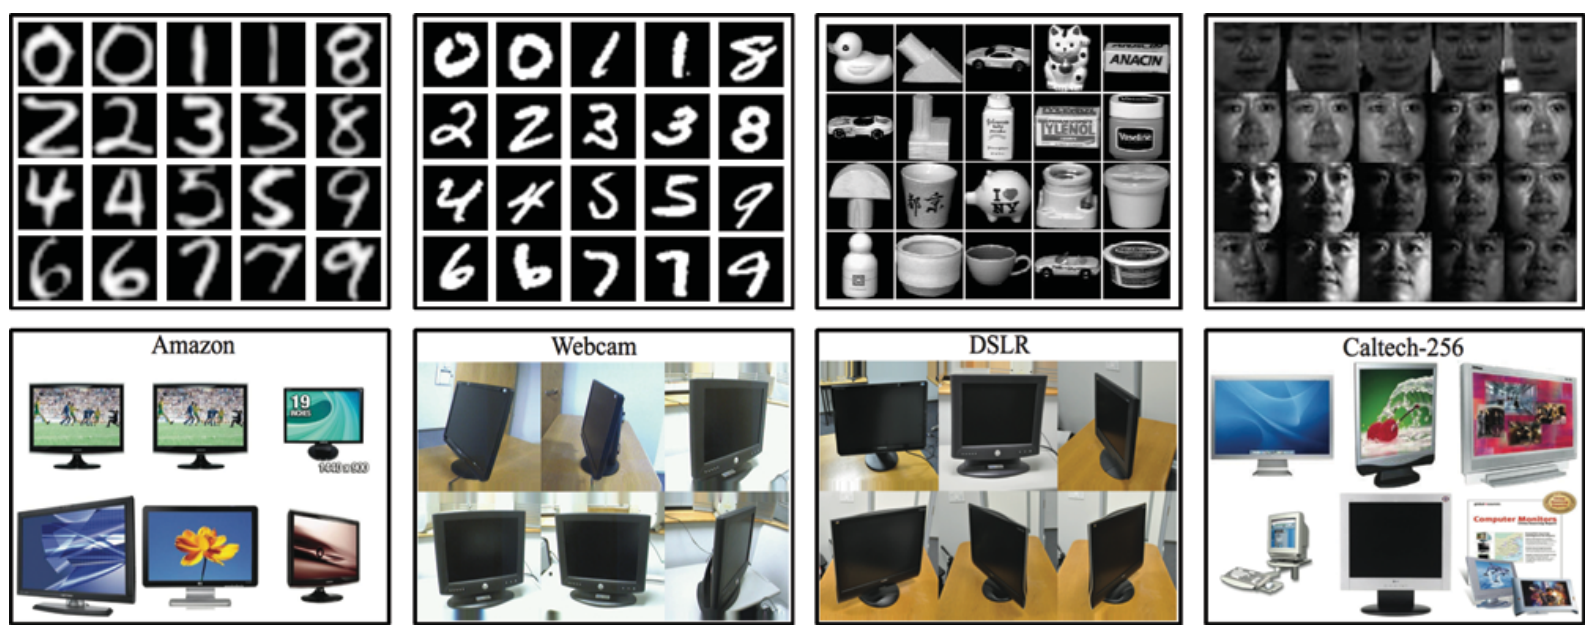
\includegraphics[height=0.33\textheight]{figs/d4.png}\\
\item Statistics of the six benchmark digit/face/object dataset\\ 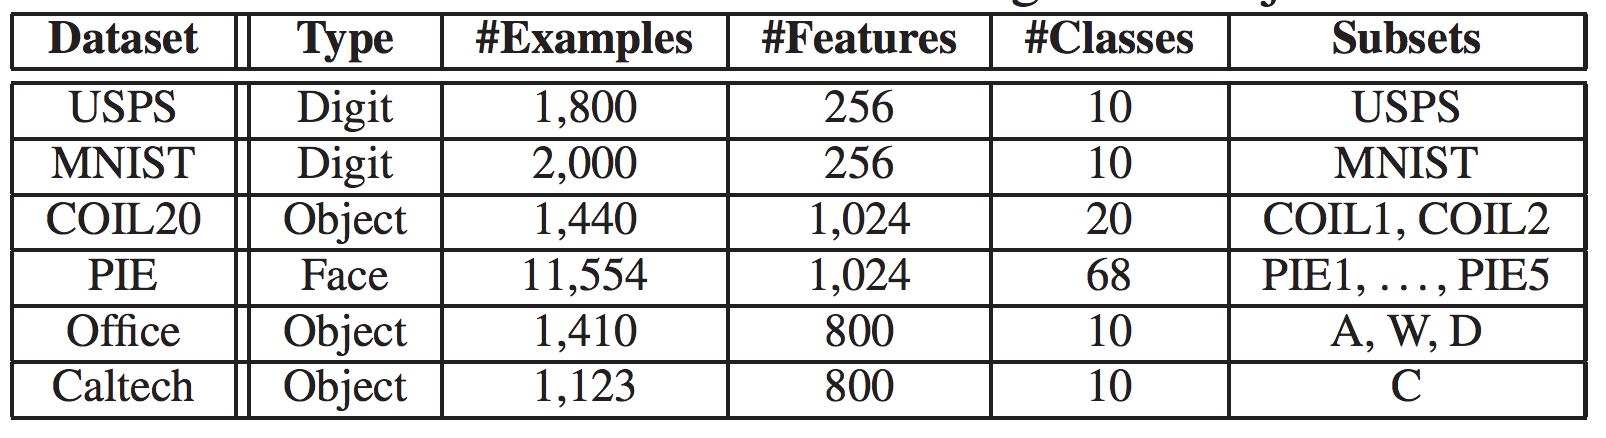
\includegraphics[height=0.3\textheight]{figs/t1.png}
\end{itemize}
\end{frame}
%==================================

\begin{frame}
{Quantitative comparisons}
\begin{columns}[totalwidth=\textwidth]
\begin{column}{\textwidth}
\tcboxfit[height=0.9\textheight]{
\begin{block}
{Evaluation}
\begin{equation}\label{eq:accuracy}
	\begin{array}{c}
		Accuracy = \frac{{\left| {x:x \in {D_T} \wedge \hat y(x) = y(x)} \right|}}{{\left| {x:x \in {D_T}} \right|}}
	\end{array}
\end{equation}
where ${\cal{D_T}}$ is the target domain treated as test data, ${\hat{y}(x)}$ is the predicted label and ${y(x)}$ is the ground truth label for a test data  $x$.
\end{block}
\begin{block}
{Domain adaptation task:}
\begin{itemize}
\item USPS \emph{vs} MINIST: 2; COIL1 \emph{vs} COIL2: 2
\item PIE:   $5 \times 4 = 20$ cross-domain face datasets, e.g., PIE1 \emph{vs} PIE2,
PIE1 \emph{vs} PIE3,...
\item office+Caltech:  $ 4\times3 = 12$ cross-domain object datasets, e.g., C $\rightarrow$ A, C $\rightarrow$W, C $\rightarrow$ D,..., D $\rightarrow$ W.
\end{itemize}
\end{block}
% \begin{block}
% {Baseline methods }
% \begin{itemize}
% \item (1)1-Nearest Neighbor Classifier(NN); 
% \item (2) Principal Component Analysis (PCA) +NN; \item (3) Geodesic Flow Kernel(GFK) \footcite{gong2012geodesic} + NN; 
% \item (4) Transfer Component Analysis(TCA) \footcite{pan2011domain} +NN;
% \item (5)Transfer Subspace Learning(TSL) \footcite{4967588} +NN; 
% \item (6) Joint Domain Adaptation (JDA) \footcite{long2013transfer} +NN

% \end{itemize}

%     \end{block}

    }
    \end{column}
    \end{columns}
\end{frame}


\begin{frame}
{Quantitative comparisons}
\begin{columns}[totalwidth=\textwidth]
\begin{column}{\textwidth}
\tcboxfit[height=0.9\textheight]{
\begin{block}
{Baseline methods }
\begin{itemize}
\item (1)1-Nearest Neighbor Classifier(NN); 
\item (2) Principal Component Analysis (PCA) +NN; \item (3) Geodesic Flow Kernel(GFK) \footcite{gong2012geodesic} + NN; 
\item (4) Transfer Component Analysis(TCA) \footcite{pan2011domain} +NN;
\item (5)Transfer Subspace Learning(TSL) \footcite{4967588} +NN; 
\item (6) Joint Domain Adaptation (JDA) \footcite{long2013transfer} +NN
\item (7) CDDA(a): JDA + repulsive term +NN
\item (8) CDDA(b): CDDA(a)+ Label deduction

\end{itemize}

    \end{block}

    }
    \end{column}
    \end{columns}
\end{frame}

\begin{frame}
{Quantitative comparisons}
\begin{columns}[totalwidth=\textwidth]
\begin{column}{\textwidth}
\tcboxfit[height=0.8\textheight]{
\begin{block}
{Quantitative comparisons I}
\begin{table}[h!]
	\centering
	\label{tab:acc}
    \resizebox{0.9\columnwidth}{!}{%
		\begin{tabular}{|l |c |c |c| c |c |c | c| c|}\hline	
			Datasets& {NN} & {PCA} & {GFK} & {TCA} & {TSL}  & {JDA} & \textbf{CDDA(a)} & \textbf{CDDA(b)} \\
			USPS \emph{vs} MNIST& 44.70&	44.95&	46.45&	51.05& 53.75&	59.65&	62.05&	\textbf{ 70.75}
			\\
			MNIST \emph{vs} USPS& 65.94&	66.22&	67.22&	56.28&	66.06&	67.28&	76.22&	\textbf{ 82.33}
			\\
			\hline
			COIL1 \emph{vs} COIL2& 83.61&	84.72&	72.50&	88.47&	88.06&	89.31&	91.53&	\textbf{ 99.58}
			\\
			COIL2 \emph{vs} COIL1& 82.78&	84.03&	74.17&	85.83&	87.92&	88.47&	93.89&	\textbf{ 99.72}
			\\
			\hline		
      \end{tabular}}
	\end{table}
    \end{block}
    \begin{itemize}
    \item  It is worth noting  that the proposed  CDDA depicts $\bf 99.65$ accuracy on \textbf{COIL20}; 
    \item This is rather an unexpected impressive score given the unsupervised nature of the domain adaptation for the target domain.
    \end{itemize}

    }
    \end{column}
    \end{columns}
\end{frame}
%=============
%=============================

\begin{frame}
{Quantitative comparisons }
\begin{columns}[totalwidth=\textwidth]
\begin{column}{\textwidth}
\tcboxfit[width=\textwidth]{
    \begin{block}{Quantitative comparisons II}
	\begin{table}[h!]
	\centering
	\label{tab:acc}
    \resizebox{0.9\columnwidth}{!}{%
		\begin{tabular}{|l |c |c |c| c |c |c | c| c|}\hline		
	Datasets& {NN} & {PCA} & {GFK} & {TCA} & {TSL}  & {JDA} & \textbf{CDDA(a)} & \textbf{CDDA(b)} \\
    C $\rightarrow$ A&  23.70&	36.95&	41.02&	38.20&	44.47&	44.78&	48.33&	\textbf{ 52.09}
			\\
			C $\rightarrow$ W&  25.76&	32.54&	40.68&	38.64&	34.24&	41.69&	44.75&	\textbf{ 47.12}
			\\
			C $\rightarrow$ D&  25.48&	38.22&	38.85&	41.40&	43.31&	45.22&	48.41&	\textbf{ 45.86}
			\\
			A $\rightarrow$ C&  26.00&	34.73&	40.25&	37.76&	37.58&	39.36&	42.12&	\textbf{ 41.32}
			\\
			A $\rightarrow$ W&  29.83&	35.59&	38.98&	37.63&	33.90&	37.97&	\textbf{41.69}&	38.31
			\\
			A $\rightarrow$ D&  25.48&	27.39&	36.31&	33.12&	26.11&	\textbf{39.49}&	37.58&	38.22
			\\
			W $\rightarrow$ C&  19.86&	26.36&	30.72&	29.30&	29.83&	31.17&	31.97&	\textbf{ 33.30}
			\\
			W $\rightarrow$ A&  22.96&	31.00&	29.75&	30.06&	30.27&	32.78&	37.27&	\textbf{ 41.75}
			\\
			W $\rightarrow$ D&  59.24&	77.07&	80.89&	87.26&	87.26&	89.17&	87.90&	\textbf{ 89.81}
			\\
			D $\rightarrow$ C&  26.27&	29.65&	30.28&	31.70&	28.50&	31.52&	\textbf{ 34.64}&	33.66
			\\
			D $\rightarrow$ A & 28.50&	32.05&	32.05&	32.15&	27.56&	33.09&	33.51&	\textbf{ 33.61}
			\\
			D $\rightarrow$ W & 63.39&	75.93&	75.59&	86.10&	85.42&	89.49&	90.51&	\textbf{ 93.22}
			\\
			\hline
    \end{tabular}}
	\end{table}
    \end{block}
    }
    \end{column}
    \end{columns}
\end{frame}

\begin{frame}
{Quantitative comparisons }
\begin{columns}[totalwidth=\textwidth]
\begin{column}{\textwidth}
\tcboxfit[width=0.8\textwidth]{
    \begin{block}{Deep learning}
	\begin{table}[h!]
	\centering
	\label{tab:acc}
    \resizebox{0.7\columnwidth}{!}{%
		\begin{tabular}{|l |c |c |c| c |}\hline	
	Datasets& \textbf{CDDA(b)}& DDC \footcite{tzeng2014deep} & DAN \footcite{long2015learning}& - \\
    C $\rightarrow$ A& \textbf{ 52.09} &92.0&92.0&-
			\\
			C $\rightarrow$ W&  \textbf{ 47.12}&95.4&92.0&-
			\\
			C $\rightarrow$ D&  \textbf{ 45.86}&-&90.5&-
			\\
			A $\rightarrow$ C& \textbf{ 41.32}&-&86.0&-
			\\
			A $\rightarrow$ W& 	38.31&59.4&68.5&-
			\\
			A $\rightarrow$ D&	38.22&-&67.0&-
			\\
			W $\rightarrow$ C&  	\textbf{ 33.30}&-&81.5&-
			\\
			W $\rightarrow$ A& 	\textbf{ 41.75}&-&53.1&-
			\\
			W $\rightarrow$ D&  \textbf{ 89.81}&96.3&99.0&-
			\\
			D $\rightarrow$ C& 		33.66&-&82.0&-
			\\
			D $\rightarrow$ A & \textbf{ 33.61}&-&54.0&-
			\\
			D $\rightarrow$ W & \textbf{ 93.22}&- &96.0&-
			\\
			\hline
    \end{tabular}}
	\end{table}
    \end{block}
    }
    \end{column}
    \end{columns}
\end{frame}

%====================
\begin{frame}
{Quantitative comparisons }
\begin{columns}[totalwidth=\textwidth]
\begin{column}{\textwidth}
\tcboxfit[width=\textwidth]{
    \begin{block}{Quantitative comparisons III}
	\begin{table}[h!]
	\centering
	\label{tab:acc}
    \resizebox{0.8\columnwidth}{!}{%
		\begin{tabular}{|l |c |c |c| c |c |c | c| c|}\hline		
	Datasets& {NN} & {PCA} & {GFK} & {TCA} & {TSL}  & {JDA} & \textbf{CDDA(a)} & \textbf{CDDA(b)} \\
    \hline
   PIE1 \emph{vs} PIE2&  26.09&	24.80&	26.15&	40.76&	44.08&	58.81&	60.22&	\textbf{ 65.32}
			\\
			PIE1 \emph{vs} PIE3&  26.59&	25.18&	27.27&	41.79&	47.49&	54.23&	58.70&  \textbf{   62.81}
			\\
			PIE1 \emph{vs} PIE4 & 30.67&29.26&	31.15&	59.63&	62.78&\textbf{84.50}& 83.48& 83.54
			\\
			PIE1 \emph{vs} PIE5&   16.67&	16.30&	17.59&	29.35&	36.15&	49.75&	54.17&	\textbf{ 56.07}
			\\
			PIE2 \emph{vs} PIE1&   24.49&	24.22&	25.24&	41.81&	46.28&	57.62&	62.33&	\textbf{ 63.69}
			\\
			PIE2 \emph{vs} PIE3&   46.63&	45.53&	47.37&	51.47&	57.60&	62.93&	\textbf{ 64.64}&	61.27
			\\
			PIE2 \emph{vs} PIE4&   54.07&	53.35&	54.25&	64.73&	71.43&	75.82&	79.90	&\textbf{ 82.37}
			\\
			PIE2 \emph{vs} PIE5&   26.53&	25.43&	27.08&	33.70&	35.66&	39.89&	44.00&	\textbf{ 46.63}
			\\
			PIE3 \emph{vs} PIE1&   21.37&	20.95&	21.82&	34.69&	36.94&	50.96&	\textbf{ 58.46}&	56.72
			\\
			PIE3 \emph{vs} PIE2&   41.01&	40.45&	43.16&	47.70&	47.02&	57.95&	\textbf{ 59.73}&	58.26
			\\
			PIE3 \emph{vs} PIE4&   46.53&	46.14&	46.41&	56.23&	59.45&	68.45&	77.20&	\textbf{ 77.83}
			\\
			PIE3 \emph{vs} PIE5&   26.23&	25.31&	26.78&	33.15&	36.34&	39.95&	\textbf{ 47.24}&	41.24
			\\
			PIE4 \emph{vs} PIE1&   32.95&	31.96&	34.24&	55.64&	63.66&	80.58&	\textbf{ 83.10}&	81.84
			\\
			PIE4 \emph{vs} PIE2&  62.68&	60.96&	62.92&	67.83&	72.68&	82.63&	82.26&	\textbf{ 85.27}
			\\
			PIE4 \emph{vs} PIE3&   73.22&	72.18&	73.35&	75.86&	83.52&	\textbf{87.25}&	86.64&	86.95
			\\
			PIE4 \emph{vs} PIE5&   37.19&	35.11&	37.38&	40.26&	44.79&	54.66&	\textbf{ 58.33}&	53.80
			\\
			PIE5 \emph{vs} PIE1&  18.49&	18.85&	20.35&	26.98&	33.28&	46.46&	48.02&	\textbf{ 57.44}
			\\
			PIE5 \emph{vs} PIE2&   24.19&	23.39&	24.62&	29.90&	34.13&	42.05&	45.61&	\textbf{ 53.84}
			\\
			PIE5 \emph{vs} PIE3&  28.31&	27.21&	28.49&	29.9&	36.58&	53.31&	52.02&	\textbf{ 55.27}
			\\
			PIE5 \emph{vs} PIE4&   31.24&	30.34&	31.33&	33.64&	38.75&	57.01&	55.99&	\textbf{ 61.82}
		
			\\
			\hline
    \end{tabular}}
	\end{table}
    \end{block}
    }
    \end{column}
    \end{columns}
\end{frame}

\begin{frame}
{Quantitative comparisons}
\begin{columns}[totalwidth=\textwidth]
\begin{column}{\textwidth}
\tcboxfit[width=\textwidth]{
    \begin{block}{Quantitative comparisons: Average}
	\begin{table}[h!]
	\centering
	\label{tab:acc}
    \resizebox{0.9\columnwidth}{!}{%
		\begin{tabular}{|l |c |c |c| c |c |c | c| c|}\hline		
	Datasets& {NN} & {PCA} & {GFK} & {TCA} & {TSL}  & {JDA} & \textbf{CDDA(a)} & \textbf{CDDA(b)} \\
    \hline
			Average (USPS)& 55.32&	55.59&	56.84&	53.67&	59.90&	63.47&	69.14&	\textbf{ 76.54}
			\\
			Average (COIL)& 83.20&	84.38&	73.34&	87.15&	87.99&	88.89&	92.71&	\textbf{ 99.65}
			\\
			Average (PIE)& 34.76&	33.85&	35.35&	44.75&	49.43&	60.24&	63.10&	\textbf{ 64.60}
			\\
			Average (Amazon)&  31.37&	39.79&	42.95&	43.61&	42.37&	46.31&	48.22&	\textbf{ 49.02}
			\\
			
			Overall Average&     37.46&	39.84&	41.19&	47.22&	49.80&	57.37&	60.12&	\textbf{ 62.02}
			\\
            \hline
    \end{tabular}}
	\end{table}
    \end{block}
    }
    
    \end{column}
    \end{columns}
\end{frame}

%=================================
\section{Future work}
\begin{frame}
{Future work}
\begin{itemize}
\item Replace exiting feature as deep feature
\item Adopt our repulsive term to deep transfer learning framework, such as DAN.\\
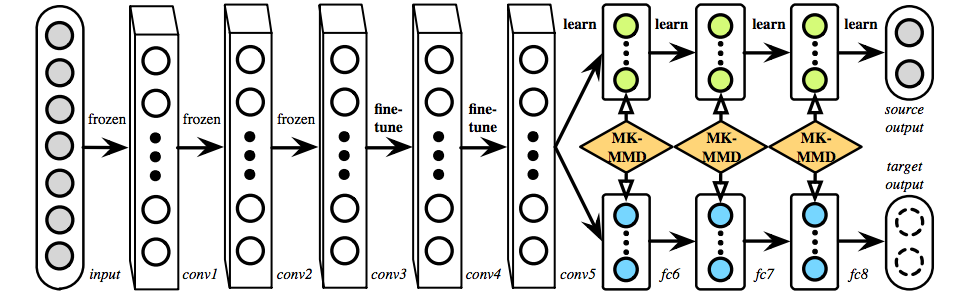
\includegraphics[width=0.8\textwidth]{figs/dan.png}
\end{itemize}
\end{frame}

%=================================
\section{References}
\begin{frame}
\begin{columns}[totalwidth=\textwidth]
\begin{column}{\textwidth}
\tcboxfit[height=0.7\textheight]{
    \begin{block}{References}
	\printbibliography
\end{block}}
\end{column}
\end{columns}
\end{frame}

\end{document}